\documentclass{standalone}
\usepackage{tikz}

\begin{document}


\hspace*{\fill}
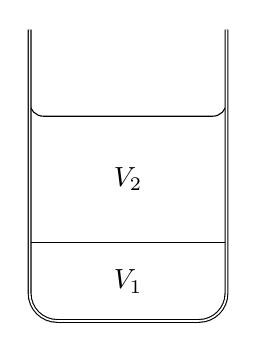
\begin{tikzpicture}
\draw[rounded corners=5] (0,2.8) --
  (0,2.6) --
  (2.5,2.6) --
  (2.5,2.8);
\draw (0,1) -- (2.5,1);
\node at (1.25,1.8) {$V_2$};
\node at (1.25,0.5) {$V_1$};
\draw[double,rounded corners=10] (0,3.7) --
  (0,0)  --
  (2.5,0)  --
  (2.5,3.7);
\end{tikzpicture}
\hspace*{\fill}
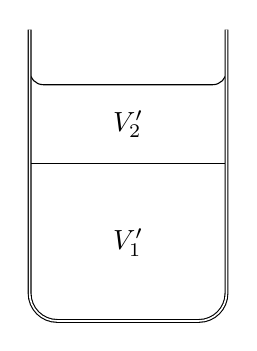
\begin{tikzpicture}
\draw[rounded corners=5] (0,3.2) --
	(0,3.0) --
	(2.5,3.0) --
	(2.5,3.2);
\draw (0,2) -- (2.5,2);	
\node at (1.25,2.5) {$V_2'$};
\node at (1.25,1) {$V_1'$};
\draw[double,rounded corners=10] (0,3.7) --
	(0,0)  --
	(2.5,0)  --
	(2.5,3.7);
\end{tikzpicture}
\hspace*{\fill}


\end{document}